\documentclass[pdflatex,compress,mathserif]{beamer}

%\usetheme[dark,framenumber,totalframenumber]{ElektroITK}
\usetheme[darktitle,framenumber,totalframenumber]{ElektroITK}

\usepackage[utf8]{inputenc}
\usepackage[T1]{fontenc}
\usepackage{lmodern}
\usepackage[bahasai]{babel}
\usepackage{amsmath}
\usepackage{amsfonts}
\usepackage{amssymb}
\usepackage{graphicx}
\usepackage{multicol}
\usepackage{lipsum}

\newcommand*{\Scale}[2][4]{\scalebox{#1}{$#2$}}%

\title{Sinyal dan Sistem}
\subtitle{Deret Fourier Waktu Diskrit}

\author{Mifta Nur Farid}

\begin{document}

\maketitle

\begin{frame}
	\frametitle{Periodic sequences}
	\begin{itemize}
		\item Sinyal waktu diskrit (sequence) $ x[n] $ dikatakan periodik jika terdapat bilangan bulat positif N di setiap
		\begin{equation}\label{eq.1}
			x[n + N] = x[n]\text{, untuk semua }n
		\end{equation}
		\item Periode dasar $ N_0 $ dari $ x[n] $ adalah bilangan bulat positif terkecil dari $ N $.
		\item Eksponensial kompleks sequence
		\begin{equation}\label{eq.2}
			x[n] = e^{j(2\pi/N_0)n} = e^{j\Omega_0 n}
		\end{equation}
		yang mana $ \Omega_0 = 2\pi / N_0 $, adalah sequence periodik dengan periode dasar $ N_0 $
	\end{itemize}
\end{frame}

\begin{frame}{Periodic Sequences}
	\begin{itemize}
		\item Perbedaan yang penting antara eksponensial kompleks waktu diskrit dengan eksponensial kompleks waktu kontinyu adalah sinyal $ e^{j\omega_0 t} $ akan berbeda untuk setiap $ \omega_0 $ yang berbeda.
		\item Namun untuk sequence $ e^{j \Omega_0 n} $, yang frekuensinya berbeda dengan kelipatan $ 2 \pi $, akan menghasilkan sequence yang identik
		\begin{equation}\label{eq.3}
			e^{j(\Omega_0 + 2 \pi k)n} = e^{j\Omega_0n} e^{j2 \pi kn} = e^{j\Omega_0n}
		\end{equation}
	\end{itemize}
\end{frame}

\begin{frame}{Periodic Sequences}
	\begin{itemize}
		\item Diketahui
		\begin{equation}\label{eq.4}
			\Psi_k[n] = e^{j k \Omega_0 n},~~\Omega_0 = \frac{2 \pi}{N_0},~~k = 0,\pm1,\pm2,\dots
		\end{equation}
		\item Kemudian berdasarkan pers. \ref{eq.3}, maka didapatkan
		\begin{equation}\label{eq.5}
			\Psi_0[n] = \Psi_{N_0}[n]~~\Psi_1[n] = \Psi_{N_0 + 1}[n]~~\cdots~~\Psi_k[n] = \Psi_{N_0} + k[n]~~\cdots
		\end{equation}
		\item atau dalam bentuk yang lebih umum
		\begin{equation}\label{eq.6}
			\Psi_k[n] = \Psi_{k+mN_0}[n]~~~m = \text{ bilangan bulat (integer)}
		\end{equation}
		\item Jadi, sequence $ \Psi_k[n] $ hanya berbeda pada rentang nilai $ N_0 $ yang berurutan dari $ k $.
	\end{itemize}
\end{frame}

\begin{frame}
	\frametitle{Representasi deret Fourier diskrit}
	\begin{itemize}
		\item Representasi deret Fourier diskrit dari sequence periodik $ x[n] $ dengan periode dasar $ N_0 $ adalah
		\begin{equation}\label{eq.7}
			x[n] = \sum\limits_{k=0}^{N_0-1} c_k e^{j k \Omega_0 n}~~\Omega_0 = \frac{2 \pi}{N_0}
		\end{equation}
		yang mana $ c_k $ adalah koefisien Fourier
		\begin{equation}\label{eq.8}
			c_k = \frac{1}{N_0} \sum_{n = 0}^{N_0 - 1} x[n] e^{-j k \Omega_0 n}
		\end{equation}
	\end{itemize}
\end{frame}

\begin{frame}{Representasi deret Fourier diskrit}
	\begin{itemize}
		\item Berdasarkan pers. \ref{eq.5} dan \ref{eq.6}, pers. \ref{eq.7} dan \ref{eq.8} dapat ditulis kembali menjadi
		\begin{equation}\label{eq.9}
			x[n] = \sum\limits_{k = <N_0>} c_k e^{jk\Omega_0n}~~~\Omega_0 = \frac{2\pi}{N_0}
		\end{equation}
		\begin{equation}\label{eq.10}
			c_k = \frac{1}{N_0} \sum_{n = <N_0>} x[n]e^{jk\Omega_0n}
		\end{equation}
	\end{itemize}
\end{frame}

\begin{frame}{Representasi deret Fourier diskrit}
	\begin{itemize}
		\item[] yang mana $ \sum_{k = <N_0>} $ menunjukkan bahwa penjumlahan ada pada $ k $ karena $ k $ bervariasi pada rentang $ N_0 $ bilangan bulat (integer) yang berurutan.
		\item Pengaturan $ k = 0 $ dalam pers. \ref{eq.10}, kita dapatkan
		\begin{equation}\label{eq.11}
			c_0 = \frac{1}{N_0} \sum_{n = <N_0>} x[n]
		\end{equation}
		mengindikasikan bahwa $ c_0 $ sama dengan nilai rata-rata dari $ x[n] $ selama suatu periode.
		\item Koefisien Fourier $ c_k $ sering disebut sebagai koefisien spektral dari $ x[n] $
	\end{itemize}
\end{frame}

\begin{frame}
	\frametitle{Latihan soal}
	\begin{enumerate}
		\item Tentukan koefisien Fourier dari sequence periodik $ x[n] $ yang ditunjukkan oleh gambar di bawah ini
	\end{enumerate}
	\begin{center}
		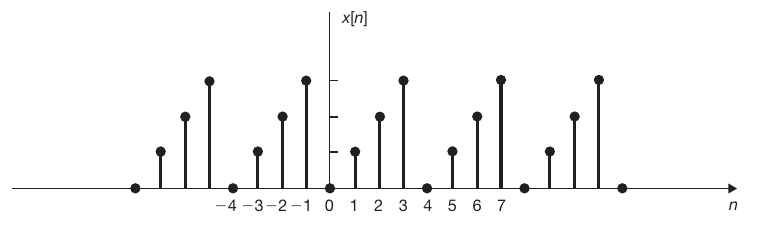
\includegraphics[width=\linewidth]{img/img01}
	\end{center}
	
\end{frame}

\end{document}
